%!TEX root = main.tex
\tvcg{\section{Understanding Scientific Data Analysis (RQ1)}}
%\cut{ \subsection{Understanding Scientific Data Analysis}
\par Our initial inspiration for building a VQS came from informal discussions with many academic and industry analysts. Their current workflows required the analysts to manually examine a large number of visualizations to derive insights from their data. In this section, we address RQ1 by understanding the limitations and opportunities in existing scientific data analysis workflows in three research areas. We begin by describing the participants in these areas.
\subsection{Participants, Datasets and Workflows}
We recruited participants by reaching out to research groups who were interested in using VQSs for exploring their data via email. %\kk{Need to be more explicit about recruitment strategy here?}
\tvcg{As we will describe in Section \ref{metastudy}, we initially spoke to analysts from 12 different potential application areas and narrowed down to three use cases in astronomy, genetics, and material science for our participatory design study.} We summarize the common properties of and differences between these three groups of researchers in Figure~\ref{example} and describe the desirable characteristics common to these datasets that make them suitable for VQSs in Section~\ref{metastudy}.
\par Six scientists from three research groups participated in the design of \zv. The evaluation study participants included these six scientists, along with three ``blank-slate'' participants who had never encountered \zv before. While participatory design subjects actively provided feedback on \zv with their data, they only saw us demonstrating their requested features and explaining the system to them, rather than actively using the system on their own. So the evaluation study was the first time that all nine of the participants used \zv to explore their datasets. On average, the participants had more than 8 years of research experience working in their respective fields. We list the participants in Table~\ref{participants}, and will refer to them by their anonymized ID as listed in the table throughout the paper. 
\begin{table}[h]
\centering
\vspace{-10pt}
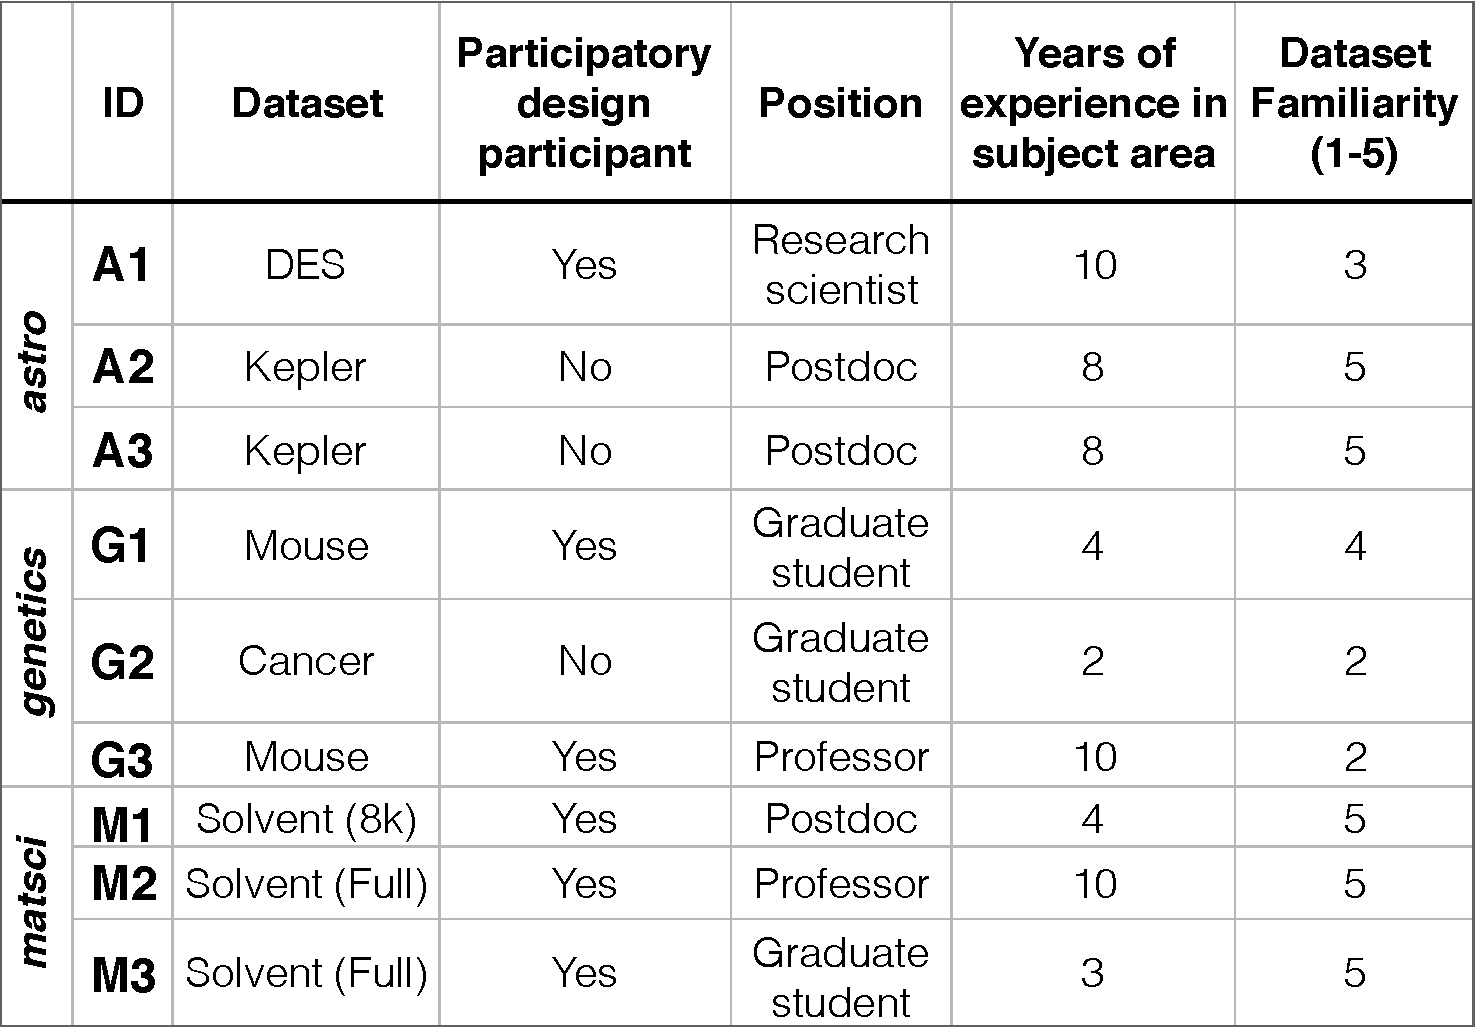
\includegraphics[width=\linewidth]{figures/participants.pdf}
\caption{Participant information. The Likert scale used for dataset familiarity ranges from 1 (not at all familiar) to 5 (extremely familiar).}
\label{participants}
\vspace{-10pt}
\end{table}
\par The research questions and objectives of the participants were diverse even among those in the same subject area and using the same dataset. Examples of research questions included: 
\begin{denselist}
\item Understanding the gene expression profiles of breast cancer cells that exhibit induced, transient, and  repressed patterns after a particular treatment.
\item Studying common patterns among stars that exhibit planetary transits versus stars that do not, from the Kepler space telescope\footnote{\url{www.nasa.gov/mission_pages/kepler/main/index.html}}.
\item Identifying battery solvents with favorable properties and mass production potential through studying how changes in certain chemical properties correlate with changes in other chemical properties. \end{denselist}
The pre-study survey with the participants showed that out of all of the steps in their data analysis workflow\footnote{This includes viewing and browsing data, data cleaning and wrangling, computing statistics, data visualization, and model building or machine learning.}, they spend the most time computing statistics and creating visualizations.
The main bottlenecks cited in their existing workflows included the challenge of dealing with large amounts of data, writing custom processing and analysis scripts, and long turnaround times incurred by making modifications to an upstream operation in a segmented workflow. %\ccut{On average, participants expressed interest in adopting \zv in their day-to-day workflow as eight from a Likert scale of ten after the study \kk{not sure what this means}.}
\begin{figure*}[ht!]
\centering
\vspace{-10pt}
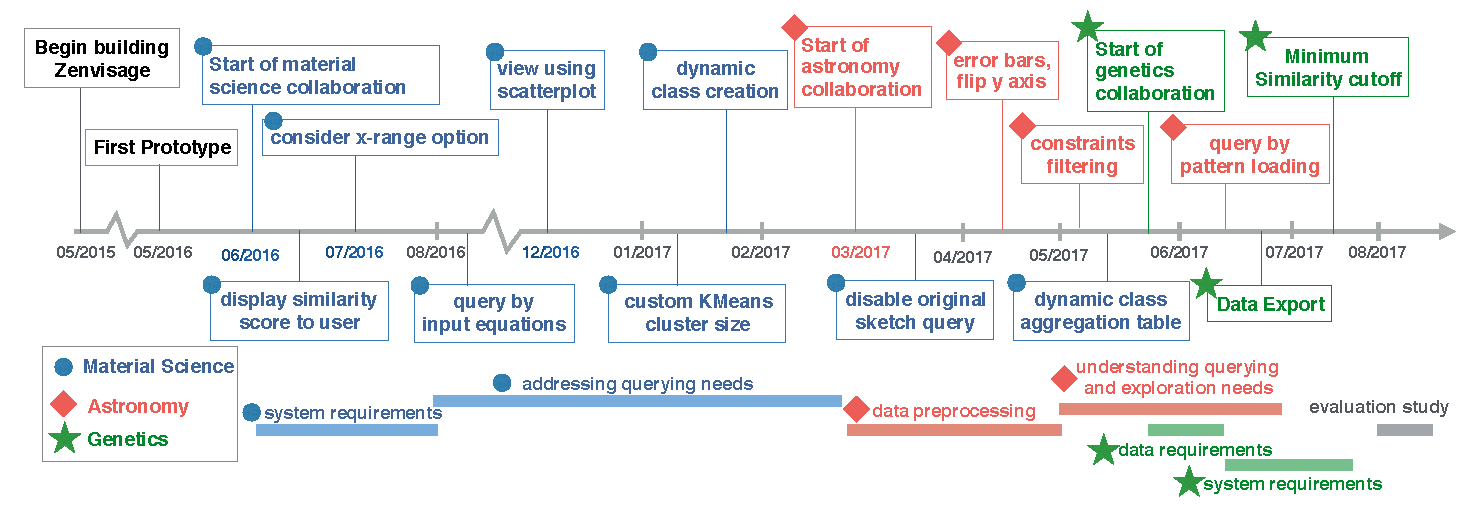
\includegraphics[width=6in]{figures/timeline_new.pdf}
\vspace{-6pt}\caption{Participatory design timeline for the scientific use cases.}
\label{timeline}
\vspace{-10pt}
\end{figure*}
\par During the participatory design process, we collaborated with each of the teams closely with an average of two meetings per month, where we learned about their datasets, objectives, and how VQSs could help address their research questions. A detailed timeline of our engagement with the participants and the features inspired by their use cases can be found in Figure \ref{timeline}. Participants provided datasets they were exploring from their domain, whereby they had a vested interest to use a VQS to address their own research questions. We  describe the three scientific use cases below.

\stitle{Astronomy (\astro):} The Dark Energy Survey (DES) is a multi-institutional project with over 400 scientists. Scientists use a multi-band telescope that takes images of 300 million galaxies over 525 nights to study dark energy\cite{Drlica-Wagner2017}. The telescope also focuses on smaller patches of the sky on a weekly interval to discover astrophysical transients (objects whose brightness changes dramatically as a function of time), such as supernova explosions or quasars. The output is a time series of brightness observations associated with each object extracted from the images observed. %\kk{is it 4 years of 525 nights?}\dor{it's a bit confusing, because they only observe half a year on the southern hemisphere, will skip talking about this} 

For over five months, we worked closely with an astronomer on the project's data management team working at a supercomputing facility. \ccut{We also gathered feedback from other astronomers who were interested in studying the properties of astrophysical transients during a collaboration-wide meeting.} The scientific goal is to identify a smaller set of potential candidates that may be astrophysical transients in order to study their properties in more detail. These insights can help further constrain physical models regarding the formation of these objects.

\stitle{Genetics (\bio):} Gene expression is a common data type used in genomics and is obtained via microarray experiments. \techreport{In these experiments, a grid containing thousands of DNA fragments are exposed to stimuli and measurements for the level at which a gene is expressed are recorded as a function of time.} The data used in the participatory design sessions was the gene expression data over time for mouse stem cells aggregated over multiple experiments, downloaded from an online database\footnote{\url{ncbi.nlm.nih.gov/geo/}}. 
\par  We worked with \tvcg{a graduate student and a PI} at a research university over three months who were using gene expression data to better understand how genes are related to phenotypes expressed during early development~\cite{Peng2016,Gloss2017}. They were interested in using \zv to cluster gene expression data before conducting analysis with a downstream machine learning workflow. 

\stitle{Material Science (\matsci):} We collaborated with material scientists at a research university who are working to identify solvents that can improve battery performance and stability. These scientists work with large datasets containing over 25 chemical properties for more than 280,000 different solvents obtained from simulations. \techreport{Once they have identified a solvent that also produces favorable results in an experiment, they identify other solvents with similar properties,  which may be cheaper or safer to manufacture at an industrial scale.}
\par We worked closely with a graduate students, a postdoctoral researcher, and a PI for over a year to design a sensible way of exploring their data using VQSs\footnote{Note that while we have interacted with the \matsci participant during the initial development stage, the participatory design formally started in June 2016}. Each row of their dataset represents a unique solvent, and consists of 25 different chemical attributes. They wanted to use \zv to identify solvents that have similar properties to known solvents but are more favorable (e.g. cheaper or safer to manufacture), and identify how changes in certain chemical attributes affects them.
\raggedbottom
%%%%%%%%%%%%%%%%%%%%%%%%%%%%%%%%%
\subsection{Cognitive Walkthrough Sessions}
\tvcg{During the design study, we observed the participants as they conducted a cognitive walkthrough demonstrating every component of their current data analysis workflow. Cognitive walkthroughs highlight the existing workflows and behavior that participants have adopted for conducting certain tasks~\cite{Nielsen1994}.}
\techreport{
	\begin{figure}[ht!]
		\centering
		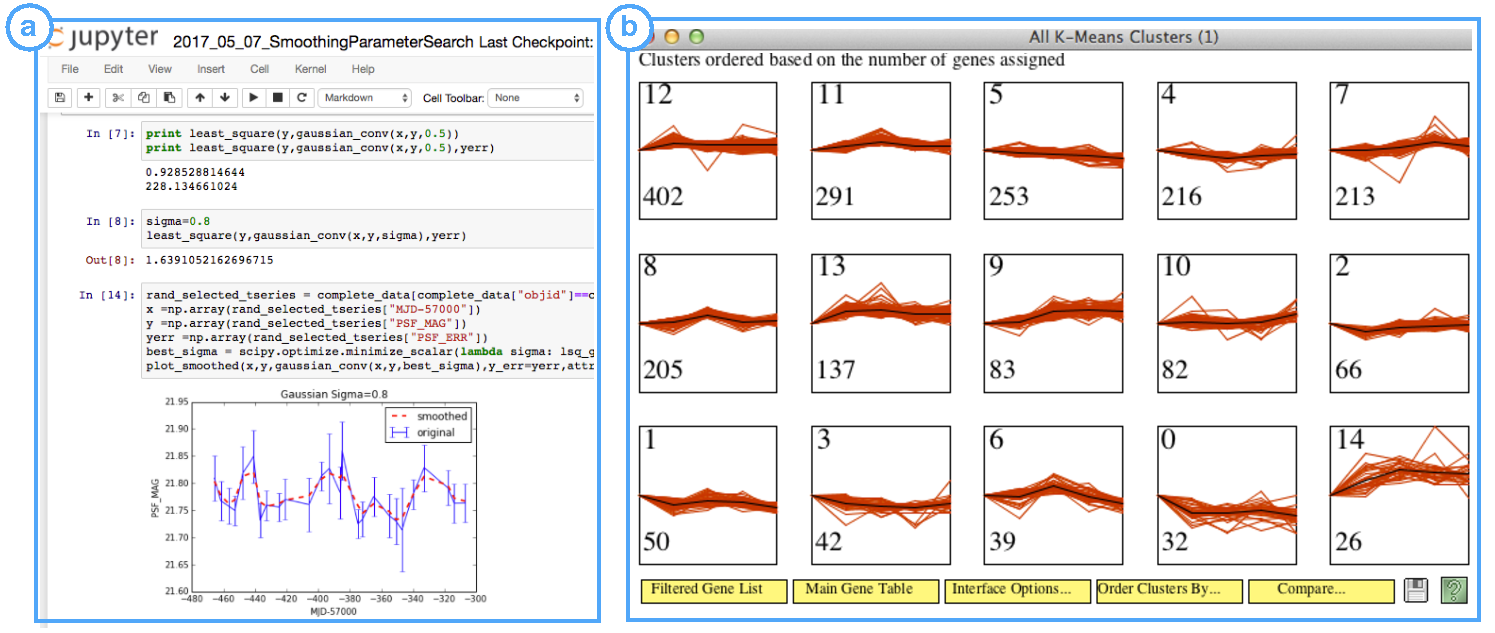
\includegraphics[width=\linewidth]{figures/workflow.pdf}
		\caption{Examples of the scientists' original workflow: a) The astronomer performs various data analysis task using the Jupyter notebook environment, b) The geneticists uses a domain-specific software to examine clustering outputs.}
		\label{workflow}
	\end{figure}
}

\stitle{Astronomy:} Since astronomical datasets are often terabytes in scale, they are often processed and stored in highly specialized data management centers in supercomputing centers. The collaboration's data management team has created a command-line interface that enables users to easily query, browse, and download their data\techreport{\footnote{ \url{github.com/mgckind/easyaccess}}}. 
After the data is downloaded, most of the work is done programmatically through Python in an interactive Jupyter notebook environment\footnote{\url{jupyter.org}}. The astronomer inspects the data schema, performs data cleaning and  wrangling, computes relevant statistics, and generates visualizations to search for anomalies or objects of interest, as shown in Figure \ref{workflow}a.
\par While an experienced astronomer who has examined many transient light curves can often distinguish an interesting transient object from noise by sight, they must visually examine and iterate through large numbers of visualizations of candidate objects. Manual searching is time-consuming and error prone as the majority of the objects will not be astronomical transients.
Participant A1 was interested in \zv as he recognized how specific pattern queries could help scientists directly search for these rare objects. 
\ccut{\dor{we can probably cut this paragraph out} \techreport{\par If an object of interest or region is identified through the visual analysis, then the astronomer may be interested in inspecting the image of the region for cross-checking that the significant change in brightness of the object is not due to an imaging artifact. This could be done using a custom built web-interface that facilitates the access of cutout images for a queried region of the sky.}}

\stitle{Genetics:} Participant G1 processes the raw microarray data by using a preprocessing script written in R\techreport{, where she (i) sub-selects 144 genes of interest, (ii) cleans up an experimental artifact due to measurements on multiple probes, (iii) log-transforms the raw data to show a more distinct shape profile for clustering, (iv) normalizes the gene expression values into the range of 0 to 1, and (v) performs Loess smoothing with default parameters to reduce the noise in the data}. To analyze the data, the preprocessed data is loaded into a desktop application for visualizing and clustering gene expression data\footnote{ \url{www.cs.cmu.edu/~jernst/stem/}}. G1 sets several clustering and visualization parameters on the interface before pressing a button to execute the clustering algorithm. The cluster visualizations are then displayed as overlaid time series for each cluster, as shown in the visualization in Figure \ref{workflow}b. G1 visually inspects that all the patterns in each cluster look ``clean'' and checks the number of outlier genes that do not fall into any of the clusters.  If the number of outliers is high or the visualizations look unclean, she reruns the clustering by increasing the number of clusters. Once the visualized clusters look ``good enough'', G1 exports the cluster patterns into a csv file to be used as features in their downstream regression tasks.
\par Prior to the study, the student (G1) and PI (G3) spent over a month attempting to determine the best number of clusters for their upstream analysis based on a series of static visualizations and statistics computed after clustering. While regenerating their results took no more than 15 minutes every time they made a change, the multi-step, segmented workflow meant that all changes had to be done offline, so that valuable meeting time was not wasted trying to regenerate results. The team had a vested interest in participating in the design of \zv as they saw how the interactive nature of VQSs and the ability to query other time series with clustering results could dramatically speed up their collaborative analysis process. 

\stitle{Material Science:} Participant M1 starts his data exploration process with a list of known and proven solvents as a reference. For instance, he would search for solvents which have boiling point over 300 Kelvins and the lithium solvation energy under 10 kcal/mol using basic SQL queries. This would help him narrow down the list of solvents, and he would continue this process with other properties. The scientist also considers the availability and the cost of the solvents while exploring the dataset. When the remaining list of the solvents is sufficiently small, he drills down to more detail (e.g., such as looking at the chemical structure of the solvents to consider the feasibility of conducting experiments with the solvent). While he could identify potential solvents through  manual lookup and comparison,  the process lacked the ability to reveal complicated trends and patterns that might be hidden, such as how the change in one attribute can affect the behavior of other attributes of a solvent. M1 was interested in using a VQS as it was infeasible for him to manually compare between large numbers of solvents and their associated properties manually.
\raggedbottom